\begin{frame}{deliberate scheduling}
\begin{itemize}
\item so far: 
    \begin{itemize}
    \item devices decide when to try to send
    \item channel supporting one transmitter
    \end{itemize}
\vspace{.5cm}
\item alternate idea (cellular networks): divide
\item several available channels
    \begin{itemize}
    \item typically different frequencies
    \item signal encoding chosen to avoid interference between close frequencies
    \end{itemize}
\item slots within each time interval
\end{itemize}
\end{frame}

\begin{frame}

{\fontsize{9}{10}\selectfont Computer Networks: A Systems Approach, Figure 54}
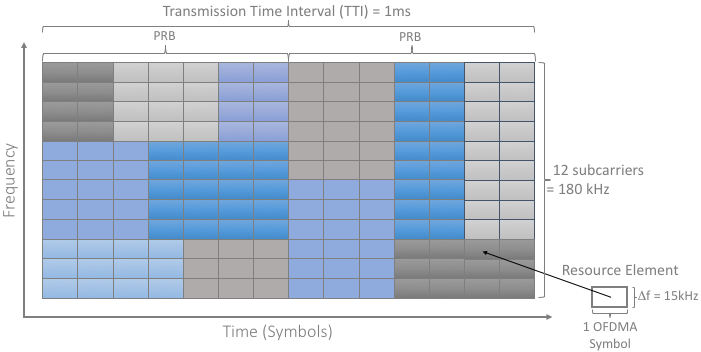
\includegraphics[width=\textwidth]{../multiaccess/CNSA-Fig54}
\end{frame}

\begin{frame}{central scheduler idea}
    \begin{itemize}
    \item `base stations' track active user devices
    \item users have bandwidth reservations
    \vspace{.5cm}
    \item base stations send out schedule of slots every $\sim$ 0.1--1ms
    \item protocol for handoff between base stations
    \item devices send back quality feedback to aid scheduling
    \end{itemize}
\end{frame}

\begin{frame}{exercise}
    \begin{itemize}
    \item central scheduling v carrier-sense
    \vspace{.5cm}
    \item exercise: which handles better\ldots
        \begin{itemize}
        \item utilizing the most of the available bandwidth
        \item independently controlled access points/base stations
        \item communications between two nearby nodes
        \end{itemize}
    \end{itemize}
\end{frame}
